% !TeX root = ../dokumentation.tex

\chapter{Projekt Ergebnisse}

\section{Erreichte Ziele}

\section{Analyse der organisatorischen Änderungen}

\subsection{WIP-Limits}
Zu Anfang des Projektes wurden sehr hohe Initialwerte für die \ac{WIP}-Limits gesetzt.
Das Problem hiermit verdeutlicht sich am besten an der \enquote{Needs Review} Swimlane.
Wie sich in Abbildung \ref{fig:WIP} (dem \ac{WIP}-Chart des Projektes) zeigt, hingen zum Anfang des ersten Sprints ein Großteil der Stories in diesem Status.

\begin{figure}
    \centering
    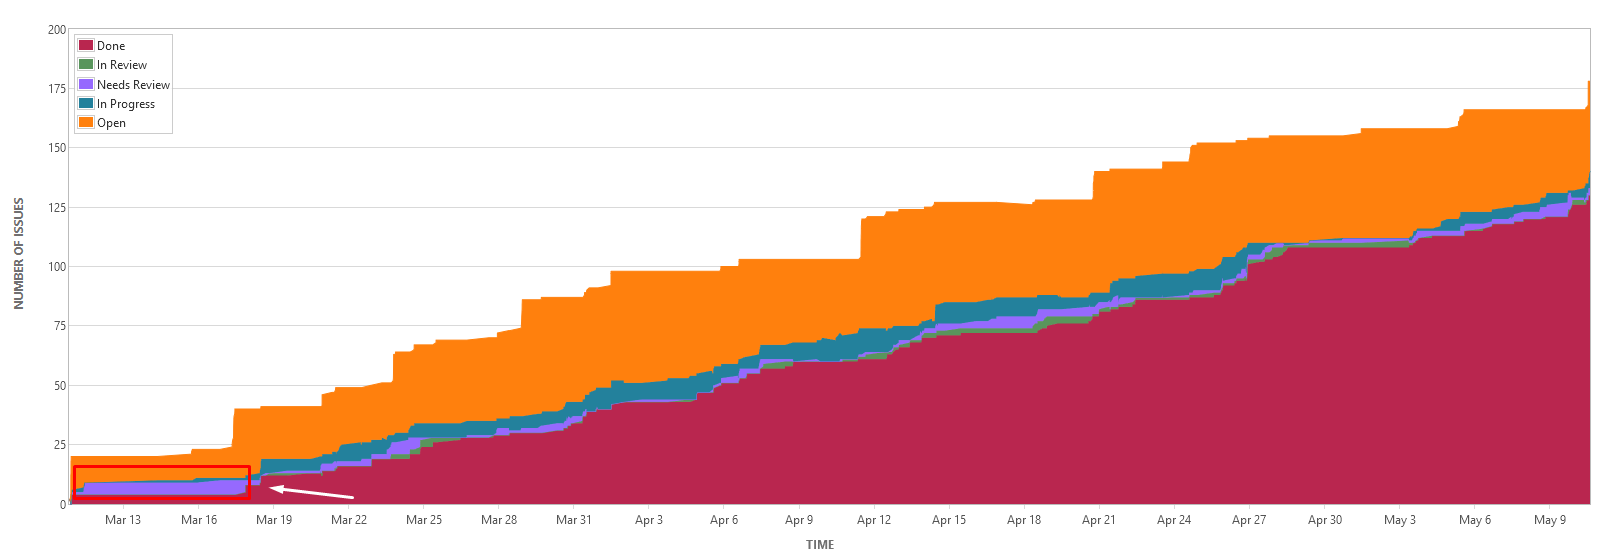
\includegraphics[width=\linewidth]{WIP-Chart.png}
    \caption{WIP Chart des Projektes}
    \label{fig:WIP}
\end{figure}

Als jedoch das \ac{WIP}-Limit dieser Swimlane von 11 auf 4 verringert wurde, ist die Aufhäufung an Tickets dem Team deutlicher geworden.
Im \ac{WIP}-Chart ist ebenfalls eindeutig zu erkennen, dass die Häufung (im Rot umrandeten Bereich) am Anfang sehr prävalent war, sich aber schlagartig zum Zeitpunkt des Einsetzten des Limits zurückgebildet hat (siehe weißer Pfeil).

\todo{Änderungen des Ablaufes erläutern und analysieren}
\section{Personenbeiträge}
(Zusammenfassung genau beschrieben in den jeweiligen Tickets der Sprints)
